\documentclass[onecolumn, draftclsnofoot,10pt, compsoc]{IEEEtran}
\usepackage{graphicx}
\usepackage{url}
\usepackage{setspace}

\usepackage{geometry}
\geometry{textheight=9.5in, textwidth=7in}
\graphicspath{ {./Images/} }

\setlength{\parskip}{1em}
% 1. Fill in these details
\def \CapstoneTeamName{		}
\def \CapstoneTeamNumber{		45}
\def \GroupMemberOne{			Blake Hudson}
\def \GroupMemberTwo{			McIntyre Santa Cruz}
\def \GroupMemberThree{			Sean Cramsey}
\def \CapstoneProjectName{		Inventor Command Predictive Analytics}
\def \CapstoneSponsorCompany{	Autodesk, Inc}
\def \CapstoneSponsorPerson{		Andrew Faix}

% 2. Uncomment the appropriate line below so that the document type works
\def \DocType{	%Problem Statement
				%Requirements Document
				%Technology Review
				Design Document
				%Progress Report
				}
			
\newcommand{\NameSigPair}[1]{\par
\makebox[2.75in][r]{#1} \hfil 	\makebox[3.25in]{\makebox[2.25in]{\hrulefill} \hfill		\makebox[.75in]{\hrulefill}}
\par\vspace{-12pt} \textit{\tiny\noindent
\makebox[2.75in]{} \hfil		\makebox[3.25in]{\makebox[2.25in][r]{Signature} \hfill	\makebox[.75in][r]{Date}}}}
% 3. If the document is not to be signed, uncomment the RENEWcommand below
%\renewcommand{\NameSigPair}[1]{#1}

%%%%%%%%%%%%%%%%%%%%%%%%%%%%%%%%%%%%%%%
\begin{document}
\begin{titlepage}
    \pagenumbering{gobble}
    \begin{singlespace}
    	\includegraphics[height=4cm]{coe_v_spot1}
        \hfill 
        % 4. If you have a logo, use this includegraphics command to put it on the coversheet.
        %\includegraphics[height=4cm]{CompanyLogo}   
        \par\vspace{.2in}
        \centering
        \scshape{
            \huge CS Capstone \DocType \par
            {\large\today}\par
            \vspace{.5in}
            \textbf{\Huge\CapstoneProjectName}\par
            \vfill
            {\large Prepared for}\par
            \Huge \CapstoneSponsorCompany\par
            \vspace{5pt}
            {\Large\NameSigPair{\CapstoneSponsorPerson}\par}
            {\large Prepared by }\par
            Group\CapstoneTeamNumber\par
            % 5. comment out the line below this one if you do not wish to name your team
            \CapstoneTeamName\par 
            \vspace{5pt}
            {\Large
                \NameSigPair{\GroupMemberOne}\par
                \NameSigPair{\GroupMemberTwo}\par
                \NameSigPair{\GroupMemberThree}\par
            }
            \vspace{20pt}
        }
        \begin{abstract}
        % 6. Fill in your abstract    
        	 Autodesk has set out to improve user productivity within their Inventor software. With the agreement of its users, Autodesk has acquired data regarding user inputs including individual key presses and mouse travel. With this data, the team has set out to analyze the information and create a system able to predict a users next input/selection. Documentation regarding the design of such a system has been created. The design has outlined key issues including, data collection, storage, and interpretation. These come in the form of types of databases and algorithms that will be implemented. Having followed the instruction set within this document, a system where users will be able to complete projects quicker and with less keystrokes/mouse travel will be developed.  
        \end{abstract}     
    \end{singlespace}
\end{titlepage}
\newpage
\pagenumbering{arabic}
\tableofcontents
% 7. uncomment this (if applicable). Consider adding a page break.
%\listoffigures
%\listoftables
\clearpage

% 8. now you write!

\section{Introduction}
\subsection{Scope}
This design document for the Autodesk Inventor Analytics projects outlines the necessary components needed to create a functioning piece of software that is intended to improve user experience. The piece in question will be an addition to the already existing software Autodesk Inventor. This addition will make use of past key strokes to predict future inputs and in turn hasten the rate of user productivity while working with Autodesk Inventor. This document focuses on the organization and key methods that will be employed. Ultimately, this document is intended to be referenced when questions regarding design appear during implementation. This can include but is not limited to types of existing systems that will be used, algorithms or methods that will be implemented, and services that will be met. What this document does not include is how to go about implementation. This will ultimately be up to the designer, with the knowledge that any final product must clearly have been developed using this design document. 
\subsection{Purpose}
The purpose of this design document is to specify exactly how the Autodesk Inventor analytic project should be implemented. This document contains which algorithm to use, along with pertinent variable information that can be implemented in however the designer sees fit. The type of data, along with how much and for how the long the data will be stored will be defined. 
\subsection{Intended Audience}
The audience for which this design document is intended are technical and managerial stakeholders. This document should be a clear and concise guide for developers to create the addition to Autodesk Inventor. Should a supervisor need explanation the document is designed so that a developer can quickly point to the section that guided their decision. This is also meant for the developers to find themselves with little to no questions on design decisions. 
\subsection{Conformance}
A product will conform if it meets all the requirements defined within this document. Requirements will therefore be clearly identifiable and enumerable. Particular requirements are defined as stretch goals and will not be expected in the final product. 
\null\newpage
\section{Definitions}
\begin{itemize}
\item Autodesk Inventor - A CAD software used in mechanical design and product simulation.
\item Analytics - Discovery, interpretation, and communication of meaningful patterns in data and applying those patterns towards effective decision making.
\item Add-in - A piece of software that adds to the core functionality of the Autodesk Inventor software.
\item CAD - Computer Aided Design technologies.
\item UI - User Interface
\item JSON - JavaScript Object Notation is a lightweight data-interchange format. It is easy for humans to read and write. It is easy for machines to parse and generate.
\item XML - Extensible Markup Language, a metalanguage which allows users to define their own customized markup languages.
\item Metadata - Data which describes qualities of main data entries.
\item Tensorflow - an open source software library for high performance numerical computation. Its flexible architecture allows easy deployment of computation across a variety of platforms (CPUs, GPUs, TPUs), and from desktops to clusters of servers to mobile and edge devices. Originally developed by researchers and engineers from the Google Brain team within Google’s AI organization, it comes with strong support for machine learning and deep learning and the flexible numerical computation core is used across many other scientific domains.
\item IDE - Integrated development environment - a software application that provides comprehensive facilities to computer programmers for software development. 
\item API - Application programming interface - a set of communication protocols and tools for building software using an already developed component. 
\item RNN - Recurrent neural network - a class of artificial neural network where connections between nodes from a directed graph along a sequence. One unique feature is the dynamic behaviour surrounding time sequences. See section 7 for more details. 
\item key stroke - any recognized command sequence within Autodesk Inventor. 
\item ML/Machine Learning - A family of algorithms which use sets of data in order to perform classification or prediction problems.
\end{itemize}
\null\newpage
\section{Overview}
The Autodesk Inventor application is a CAD application that is used for design, simulation, visualization, and documentation. It has been development for twenty years and has maintained a dedicated user base. A software that has been around for decades can be difficult to update and keep customers content. Due to many issues, one being the wide variety of project types one can employ Inventor for, a software wide change to the UI failed. Due to this fact, a new approach has been commissioned where by each user of Inventor will served individually but their experiences will universally be improved. This will all be accomplished by implementing a machine learning algorithm that will keep track of a users key strokes. Once the system has reached an appropriate level of understanding, it will begin to predict and suggest to the user what their next command input will be. 

The system will be implemented using an add-in that Autodesk Inventor users will be able to download and include within their own Inventor application. The computation and storage of data will not be visible to the end-user. Ultimately there will be a visual queue that displays to the user what the system has predicted as their next input. It will not be mandatory to select the suggestion and should the user prefer to manually enter the command, the visual suggestion will not slow the user from completing their work had the add-in not been present. Selection of the suggested command will require a small amount of mouse travel along with a right click, or some single button input that the user has selected. Data collected will be stored locally and will not greatly increase the size of Inventor within a user's hard drive. 

This project is an attempt to improve a users experience while using Autodesk Inventor. Another result should be that tasks can be completed quicker due to the predictive nature of the system eliminating the need for a user to enter or look up key strokes. 
\null\newpage
\section{Model of Software System}
This section will deliver a visual representation of the relationships found within the system architecture of the Autodesk Inventor command analytics add-in. This section will give an overview of the components at work in the final solution of this product. 
\subsection{Architectural Design}
This application will be built in the form of an Inventor add-in. That is to say that the end user experience will in most cases mimic the base Inventor experience. The route of developing an add-in allows the system to access the Inventor API, as well as making changes to the U/I. Once the add-in has been installed on a user's computer any pertinent key stroke will be recorded and used to personalize the suggestions that will later be made by the system. Once the system has become satisfied with the amount of data and accuracy of prediction, it will begin to make visual suggestions to the user. This approach has been decided upon due to the ease of use versus say a separate program needing to be ran. The Add-in once downloaded will always be running as long as Inventor is running which ensures that all data collected us up to date. 
\subsection{Individual Breakdown}
\subsubsection{Data Storage}
Due to the time required in the process of training a machine learning algorithm, user data will have to be stored for a period of time in order to achieve any proficiency.  Data should be stored locally in the form of an XML, JSON or similar file format to allow for both easy debugging and machine parsing.

\subsubsection{Add-in Breakdown}
The add-in route has been chosen due to ease of accessing the API, while delivering a powerful solution that will accomplish the end goal of predictive analytics. 

\subsubsection{Design Justification}
The end goal of this application is to improve user experience and attempt to hasten the rate at which tasks can be completed while using Autodesk Inventor. To make it user friendly and have access to API along with the UI, the development of an add-in is necessary. It is simple to download and include within the Inventor directory. The add-in skips the step of opening a different application that runs in congress with Inventor. This should result in an experience for the user that looks similar to their usual interaction with Inventor, however accompanied with an added visual element that assists with project completion. 
\null\newpage
\section{Software Content}
\subsection{Data Collection}
Over the course of a user's session usage information pertaining to feature interactions will be collected and stored locally.  Relevant information could include; time of use, event trigger, and feature name. 
\subsubsection{Storage Format}
The data should be stored in a format that can be read by human testers and also be easily parsed via algorithm; existing file formats such as XML and JSON are ideal for this.
\subsection{Data Management}
The data that has been collected will be stored following an XML format. This will reduce the need for extensive over head and will be sufficient for the purposes of this project. 
\subsubsection{Usage Data}
Data collected from the user will be organized in local files and used to train the machine learning algorithm.
Over the course of multiple algorithm training sessions old information will become irrelevant and will need to be phased out of the training pool.
\subsubsection{Weight Data}
As weights are generated through training they will have to be stored locally for reference on start up of the Inventor application.  Multiple iterations can be stored to allow for a user to revert their personalized prediction set.
\subsection{Prediction}
The implemented ML algorithm will use past usage data in order to accurately determine the future behavior of a user, and make predictions that can be used by the user.
\subsection{Interface}
\subsubsection{Display}
A user will be given a simple display window which proposes 3-5 predicted commands. 
\subsubsection{Interaction}
Given these 3-5 predictions a user will have the ability to interact with the display in some manner to activate the predicted command from the interface.
\null\newpage
\section{Software perspective}
\subsection{Stakeholder Concerns}
The main concern for the development team is the accuracy of the software itself. The predictions made by the add-in need to meet a standard that has been set in order to be considered adequate. This is a proof on concept project that needs to have its underling features prove that effective results can be attained with the data provided by users. The concern for the user will include what has previously been mentioned, however a visual aspect must be present in order for them to interact with the suggestion. The user should be presented with multiple options ranging from most likely to less likely next input. 
\subsection{Viewpoints}
\subsubsection{Context}
Development of the add-in, which will complete the task of prediction of next key stroke, will focus on the accuracy of such a system. Accuracy is key to eventually improving a users experience while using Autodesk Inventor. The user base of Inventor is experienced with the current system and there are a wide variety of tasks which can be completed using the software. The developed system needs to the same experience to all of the users despite there range of practices. 
\subsubsection{Composition}
The add-in itself will address three particular needs. The first will be to house the necessary information needed to develop the suggestion. The second will be to display this to the user using the Inventor API. The third and final piece will be to again use the API but now to collect data, specifically user key inputs.  
\subsubsection{Information}
The algorithm used to generate a prediction will require the use of data in order to properly assign probabilities. The data necessary for this process will be recorded and stored locally. 
\subsubsection{Interface}
The user of Autodesk Inventor with the add-in installed and included at run time will expect a visual guide to recommendations. The visual component should list a set of possible choices, and listing them in an easy to understand manner. The user should have an option for selection that should be clear and does not override native shortcuts. 
\subsubsection{Interaction}
The add-in solution will require Inventor to be present on the machine that is being used. The add-in will run alongside Inventor, in effect mimicking a native process. The add-in should not cause performance issues due to this relationship with the overarching software. The add-in will not prevent Inventor from completing a process as it normally would without the add-in present.  
\subsubsection{Algorithm}
The algorithm will operate in such a way as to not interrupt with the user experience, and its execution will enhance the user experience.
%\section{Data Collection and Storage}
%\subsection{Collection}
%Over the course of a user session all triggered events and command calls will be collected and stored for eventual use in training the machine learning algorithm.
%\subsection{Storage}
\null\newpage
\section{Algorithm}
The algorithm is going to be a RNN. The type of problem that predicting a user command is solving is a sequential modeling problem. Where the input will be a sequence of commands and the output will be a single command. This follows a many-to-one architecture, where there are many inputs and one desired output. The RNN is modeled in figure 1.\newline
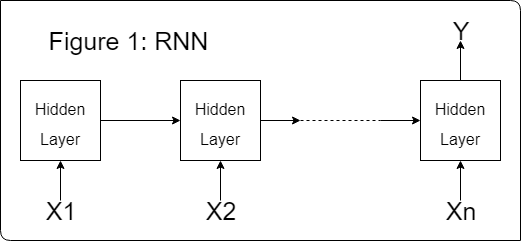
\includegraphics{RNN.png} 
\newline
In the figure above, it represents a many-to-one architecture. Where X is the input (User Commands), the square box resembles the hidden layers, and Y represents the output (predicted command). X may be any command in the Inventor IDE. There are 45 commands available in the Inventor IDE. Each user input command will be represented by the set X, for n number of commands. Each of the box's in the figure represent the hidden layer. This is where calculating the best possible answer comes from. The RNN is going to utilize two processes, forward propagation and back propagation. During the forward steps, it calculates a loss function. Which calculates a predicted output Y and compares it for accuracy. This method is called unsupervised learning. Then based on the loss function, it uses back propagation to find the and correct the error in one or many of the hidden layers. Training the neural network will be executed by those two processes. 

\null\newpage
\section{Testing}
\subsection{Functional Testing}
Unit, integration, and system testing will be carried out throughout the  development life-cycle. Unit and integration tests will be conducted more often than system tests. System tests will be carried out once more components of the add-in have been developed. The stretch goal in section nine discusses the UI integration for the add-in. If the stretch goal is achieved, interface testing will be required. It validates the UI as a business requirement. 
\subsection{Non-Functional Testing}
Performance, reliability and install testing will be conducted once the add-in is in beta. Performance testing will test the run time of the algorithm. It is necessary that the add-in does not impact the systems performance. User tests will be conducted by an experienced Inventor user. The experienced Inventor user will verify the predicted command. The purpose of this project is to enhance Inventor user experience by spending less time searching for commands. Verification will be the largest component in testing the add-ins performance.  
\null\newpage
\section{Stretch Goals}
The stretch goal will be implemented on the basis that predicting the correct command is at 80\% efficiency. Once the algorithm is proven to be efficient. The add-in will incorporate a GUI element. 

\subsection{UI Integration}
The current UI utilizes a pop-up that displays several commonly used commands. The stretch goal includes incorporating the predicted command in a similar display.  

\subsection{Machine Learning Refinements}
Not all environments that the project solution is introduced to will be the same. Some may include non-native commands or perhaps an entire different work flow. The add-in that is developed should be as dynamic as possible and serve each individual user with the same percentage of accuracy no matter the circumstance. 

\subsection{Expansion}
For the proof of concept for this command analytics project a particular section of Autodesk Inventor has been specified for use to scale down the size of the project. Should the solution prove to be effective, expansion into more regions of the Inventor software will be pursued.  


%rando extra stuff - move or delete these things as the group decides
%Storing periodic backups - maintain a history of previous coefficient values to allow for "undoing/reverting" unwanted training - experiment with blending weights; linear, bilinear etc.


\end{document}